\documentclass{beamer}
\usepackage[utf8]{inputenc}
\usetheme{Madrid}
\usecolortheme{default}
\usepackage{amsmath,amssymb,amsfonts,amsthm}
\usepackage{txfonts}
\usepackage{tkz-euclide}
\usepackage{listings}
\usepackage{adjustbox}
\usepackage{array}
\usepackage{tabularx}
\usepackage{gvv}
\usepackage{lmodern}
\usepackage{circuitikz}
\usepackage{tikz}
\usepackage{graphicx}

\setbeamertemplate{page number in head/foot}[totalframenumber]

\usepackage{tcolorbox}
\tcbuselibrary{minted,breakable,xparse,skins}



\definecolor{bg}{gray}{0.95}
\DeclareTCBListing{mintedbox}{O{}m!O{}}{%
  breakable=true,
  listing engine=minted,
  listing only,
  minted language=#2,
  minted style=default,
  minted options={%
    linenos,
    gobble=0,
    breaklines=true,
    breakafter=,,
    fontsize=\small,
    numbersep=8pt,
    #1},
  boxsep=0pt,
  left skip=0pt,
  right skip=0pt,
  left=25pt,
  right=0pt,
  top=3pt,
  bottom=3pt,
  arc=5pt,
  leftrule=0pt,
  rightrule=0pt,
  bottomrule=2pt,
  toprule=2pt,
  colback=bg,
  colframe=orange!70,
  enhanced,
  overlay={%
    \begin{tcbclipinterior}
    \fill[orange!20!white] (frame.south west) rectangle ([xshift=20pt]frame.north west);
    \end{tcbclipinterior}},
  #3,
}
\lstset{
    language=C,
    basicstyle=\ttfamily\small,
    keywordstyle=\color{blue},
    stringstyle=\color{orange},
    commentstyle=\color{green!60!black},
    numbers=left,
    numberstyle=\tiny\color{gray},
    breaklines=true,
    showstringspaces=false,
}
%------------------------------------------------------------
%This block of code defines the information to appear in the
%Title page
\title %optional
{5.3.11}

%\subtitle{A short story}

\author % (optional)
{BALU-ai25btech11017}



\begin{document}


\frame{\titlepage}
\begin{frame}{Question}
Find whether the following pair of linear equations are consistent or inconsistent:
\begin{align}
5x - 3y = 11, \quad -10x + 6y = 22
\end{align}.\\ 
\end{frame}
\begin{frame}{Theoretical Solution}
Let us solve the given equation theoretically and then verify the solution computationally \\
According to the question, \\
Given two lines\\
\begin{align}
    \Vec{A}=\begin{myvec}{5&&-3\\-10&&6}\end{myvec}\
    \Vec{B}=\begin{myvec}{11\\22}\end{myvec}\\
\end{align}
\begin{align}
    \Vec{A}\Vec{X}=\Vec{B}\
\end{align}
rank of $\Vec{A}$ =1\\
rank of $\myvec{\vec{A}&&\Vec{b}}$ =2\\
As both ranks are not equal the pair of linear equations are inconsistent
\end{frame}
\begin{frame}[fragile]
    \frametitle{C Code}

    \begin{lstlisting}
    #include <stdio.h>

int main() {
    // Coefficients of equations
    // 5x - 3y = 11  -> a1=5, b1=-3, c1=11
    // -10x + 6y = 22 -> a2=-10, b2=6, c2=22
    float a1 = 5, b1 = -3, c1 = 11;
    float a2 = -10, b2 = 6, c2 = 22;

    // Ratios
    float ratio1 = a1 / a2;
    float ratio2 = b1 / b2;
    float ratio3 = c1 / c2;

    if (ratio1 == ratio2 && ratio2 == ratio3) {
        printf("The equations are consistent and have infinitely many solutions.\n");
    } 
   

    \end{lstlisting}
\end{frame}
\begin{frame}[fragile]
    \frametitle{C Code }
    \begin{lstlisting}
 else if (ratio1 == ratio2 && ratio2 != ratio3) {
        printf("The equations are inconsistent (no solution).\n");
    } 
    else {
        printf("The equations are consistent and have a unique solution.\n");
    }

    return 0;
}
    \end{lstlisting}
\end{frame}
\begin{frame}[fragile]
    \frametitle{Python Code}
    \begin{lstlisting}
import numpy as np
import matplotlib.pyplot as plt

# Define x values
x = np.linspace(-10, 10, 400)

# First equation: 5x - 3y = 11  -> y = (5x - 11)/3
y1 = (5*x - 11)/3

# Second equation: -10x + 6y = 22 -> y = (10x + 22)/6
y2 = (10*x + 22)/6

# Plot the lines
plt.plot(x, y1, label="5x - 3y = 11")
plt.plot(x, y2, label="-10x + 6y = 22")



    \end{lstlisting}
\end{frame}

\begin{frame}[fragile]
    \frametitle{Python Code}
    \begin{lstlisting}
# Labels and title
plt.xlabel("x-axis")
plt.ylabel("y-axis")
plt.title("Graph of Linear Equations")
plt.axhline(0, color='black', linewidth=0.5)
plt.axvline(0, color='black', linewidth=0.5)
plt.grid(True, linestyle="--", alpha=0.6)

# Show legend
plt.legend()

# Save the figure
plt.savefig("lines.png", dpi=300)

# Show the plot
plt.show()

    \end{lstlisting}
\end{frame}

\begin{frame}{Plot}
    \centering
    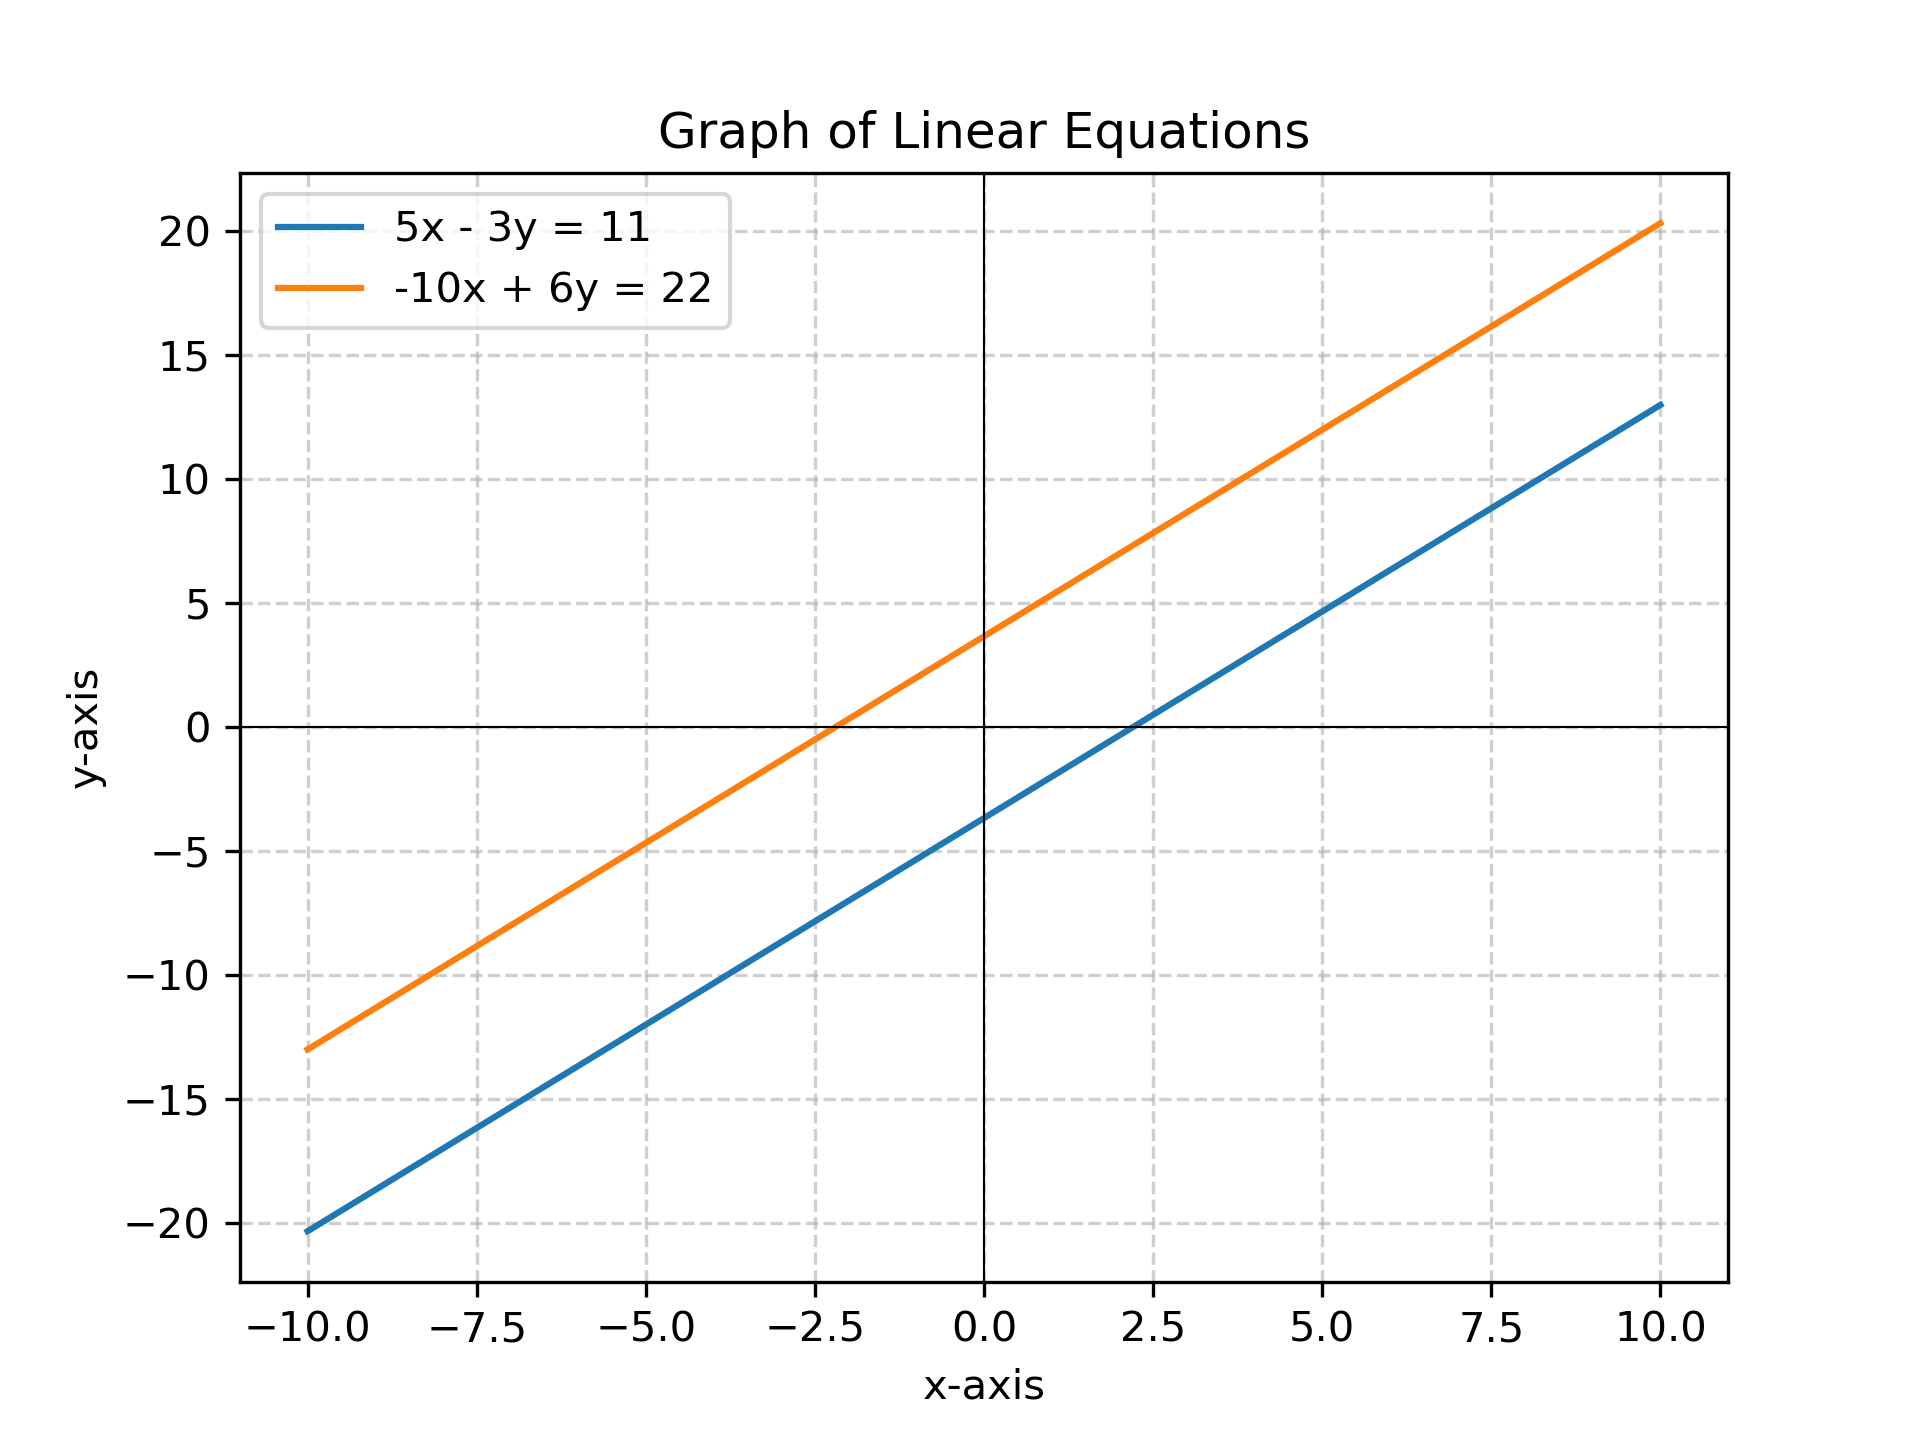
\includegraphics[width=\columnwidth, height=0.8\textheight, keepaspectratio]{figs/lines.png}     
\end{frame}




\end{document}